\section{Cech cohomology as a cohomology theory}


Let $X$ be any space, and let $K\subseteq X$ be a closed subspace.
We've defined the \v{C}ech cohomology of $K$ as the direct limit of 
$H^*(U)$ as $U$ ranges over the poset $\mathcal{U}_K$ of open neighborhoods
of $K$. This often coincides with $H^*(K)$ but will not be the same in
general. Nevertheless it behaves like a cohomology theory. To expand on
this claim, we should begin by defining a relative version. 

Suppose $L\subseteq K$ is a pair of  closed subsets of a space $X$.  Let 
$(U,V)$ be a ``neighborhood pair'' for $(K,L)$: 
\[
\begin{array}{ccc} L & \subseteq & K \\
\downsubseteq & & \downsubseteq \\
V & \subseteq & U
\end{array}
\]
with $U$ and $V$ open. These again form a directed set $\mathcal{U}_{K,L}$,
with partial order given by reverse inclusion of pairs. Then define
\[
\cHH^p(K,L)=\varinjlim_{(U,V)\in\mathcal{U}_{K,L}} H^p(U,V)\,.
\]

We will want to verify versions of the Eilenberg-Steenrod axioms for these
functors. For a start, I have to explain how maps induce maps. 

Let $\cI$ be a directed set and $A:\cI\to \mathbf{Ab}$  a functor. 
If we have an order-preserving map -- a functor -- $\varphi:\cJ\to\cI$ 
from another directed set, we get 
$A\varphi:\cJ\to\mathbf{Ab}$; so $(A\varphi)_j=A_{\varphi(j)}$.
I can form two direct limits: $\varinjlim_{\cJ}A\varphi$ and $\varinjlim_{\cI}A$. I claim that they are related by a map 
\[
\varinjlim_{\cJ}A\varphi\to\varinjlim_{\cI}A\,.
\] 
Using the universal property of direct limits, we need to come up with compatible maps $f_j:A_{\varphi(j)}\to\varinjlim_{\cI}A$. We have compatible maps 
$\inc_i:A_i\to\varinjlim_{\cI}A$ for $i\in\cI$, so we can take 
$f_j=\inc_{\varphi(j)}$. 

These maps are compatible under composition of order-preserving maps. 

\begin{example}
A closed inclusion $i:K\supseteq L$ induces an order-preserving map
$\varphi:\cU_K\to\cU_L$. The functor $H^p:\cU_K\to\mathbf{Ab}$ restricts
to $H^p:\cU_L\to\mathbf{Ab}$, so we get maps
\[
\varinjlim_{\cU_K}H^p=\varinjlim_{\cU_K}H^p\varphi\to\varinjlim_{\cU_L}H^p\,.
\]
i.e.
\[
i^*:\cHH^p(K)\to\cHH^p(L)\,.
\]
This makes $\cHH^p$ into a contravariant functor on the partially ordered 
set of closed subsets of $X$. 
\end{example}

I can do the same thing for relative cohomology, and get the maps
involved in the following two theorems, whose proofs will come in due course.
\begin{theorem}[Long exact sequence]
\label{cech-les}
Let $(K,L)$ be a closed pair in $X$. There is a long exact sequence
\begin{equation*}
\cdots\to\cHH^p(K,L)\to\cHH^p(K)\to\cHH^p(L)\xrightarrow{\delta}\cHH^{p+1}(K,L)\to\cdots
\end{equation*}
that is natural in the pair. 
\end{theorem}
\begin{theorem}[Excision]
\label{cech-excision}
Suppose $A$ and $B$ are closed subsets of a normal space, 
or compact subsets of a Hausdorff space.  
Then the map
\[
\cHH^p(A\cup B,A)\xrightarrow{\cong}\cHH^p(B,A\cap B)
\] 
induced by the inclusion is an isomorphism.
\end{theorem}

Each of these theorems relates direct limits defined over different directed 
sets. To prove them, I will want to rewrite the various direct limits
as direct limits over the same directed set. This raises the following \ldots

\begin{question}
When does $\varphi:\cJ\to\cI$ induce an isomorphism $\varinjlim_{\cJ}A\varphi\to\varinjlim_{\cI}A$?
\end{question}
This is a lot like taking a sequence and a subsequence and asking when they have the same limit. There's a cofinality condition in analysis, that has a similar expression here.
\begin{definition}
$\varphi:\cJ\to\cI$ is {\em cofinal} if for all $i\in\cI$, there exists $j\in\cJ$ such that $i\leq\varphi(j)$.
\end{definition}
\begin{example}
Any surjective order-preserving map is cofinal. 

For another example, let $(\NN_{>0},<)$ be the positive integers with their
ususal order, and $(\NN_{>0},|)$ the same set but with the divisiblity order.
There is an order-preserving map $\varphi:(\NN_{>0},<)\to(\NN_{>0},|)$ given
by $n\mapsto n!$. This map is far from surjective, but any integer $n$ 
divides some factorial ($n$ divides $n!$, for example), so $\varphi$ is cofinal. 
We claimed that both these systems produce $\QQ$ as direct limit.
\end{example}
\begin{lemma}
If $\varphi:\cJ\to\cI$ is cofinal then $\varinjlim_{\cJ}A\varphi\to\varinjlim_{\cI}A$ is an isomorphism.
\end{lemma}
\begin{proof}
Check that $\{A_{\varphi(j)}\to\varinjlim_{\cI}A\}$ satisfies the necessary and sufficient conditions to be $\varinjlim_{\cJ}A\varphi$.
\begin{enumerate}
\item For each $a\in\varinjlim_{\cI}A$ there exists $j\in\cJ$ and $a_j\in A_{\varphi(j)}$ such that $a_j\mapsto a$: We know that there exists some $i\in\cI$ and $a_i\in A$ such that $a_i\mapsto a$. Pick $j$ such that $i\leq\varphi(j)$. Then $a_i\mapsto a_{\varphi(j)}$, and by compatibility we get $a_{\varphi(j)}\mapsto a$.
\item Suppose $a\in A_{\varphi(j)}$ maps to $0\in\varinjlim_{\cI}A$. 
Then there is
some $i\in\cI$ such that $\varphi(j)\leq i$ and $a\mapsto0$ in $A_i$. 
But then there is $j'\in\cJ$ such that $i\leq\varphi(j')$, and 
$a\mapsto0\in A_{\varphi(j')}$ as well.
\end{enumerate}
\end{proof}

\begin{proof}[Proof of Theorem \ref{cech-les}, the long exact sequence]
Let $(K,L)$ be a closed pair in the space $X$. We have
\[
\cHH^p(K,L)=\varinjlim_{(U,V)\in\mathcal{U}_{K,L}}H^p(U,V)\,,
\quad
\cHH^p(K)=\varinjlim_{U\in\mathcal{U}_K}H^p(U)\,,
\quad\hbox{and}\quad 
\cHH^p(L)=\varinjlim_{V\in\mathcal{V}_L}H^p(V)\,.
\]
We can rewrite the entire sequence as
the direct limit of a directed system of exact sequences indexed by 
$\mathcal{U}_{K,L}$, since the order-preserving maps 
\[
\mathcal{U}_K \leftarrow \mathcal{U}_{K,L} \rightarrow \mathcal{U}_L 
\]
\[
U \mathrel{\reflectbox{$\mapsto$}} (U,V) \mapsto V
\]
are both surjective and hence cofinal. So the long exact sequence of a pair
in \v{C}ech cohomology is the direct limit of the system of long exact 
sequences of the neighborhood pairs $(U,V)$ and so is exact. 
\end{proof}

The proof of the excision theorem depends upon another pair of 
cofinalities.

\begin{lemma} Assume that $X$ is a normal space and $A,B$ closed subsets,
or that $X$ is a Hausdorff space and $A, B$ compact subsets.  
Then the order-preserving maps
\[
\mathcal{U}_{(A\cup B,B)} \leftarrow \mathcal{U}_A\times\mathcal{U}_B 
\rightarrow \mathcal{U}_{(A,A\cap B)}
\]
given by
\[
(W\cup Y,Y)\mathrel{\reflectbox{$\mapsto$}}(W,Y)\mapsto(W,W\cap Y)
\]
are both cofinal.
\label{lem-cofinal} 
\end{lemma}
\begin{proof}
The left map is surjective, because if $(U,V)\in\mathcal{U}_{A\cup B,B}$
then $U\in\mathcal{U}_A$, $V\in\mathcal{U}_B$, and $(U,V)=(U\cup V,V)$. 

To see that the right map is cofinal, start with 
$(U,V)\in\mathcal{U}_{A,A\cap B}$.

\medskip
\begin{center}
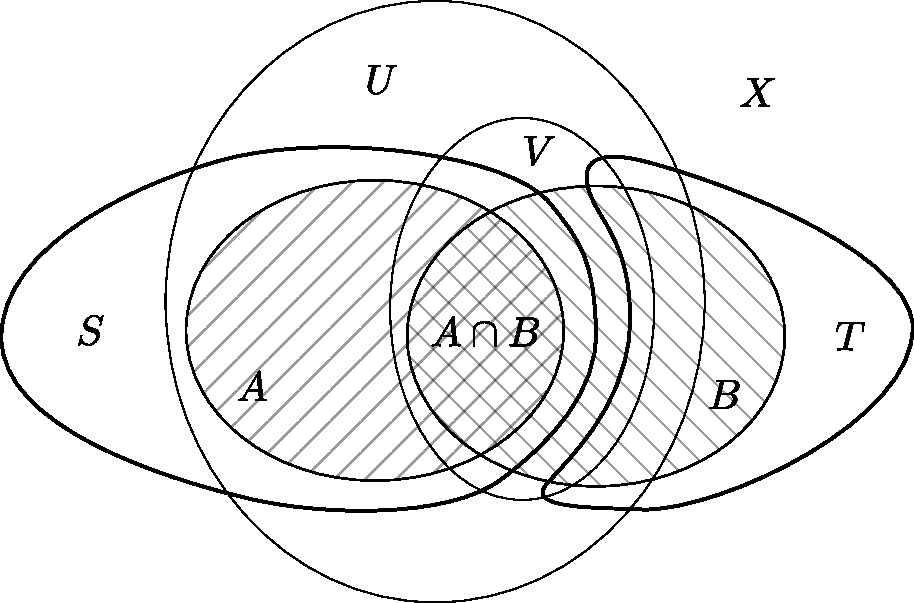
\includegraphics[width=2in]{905/Figures/35-cofinal-pair-lemma.pdf}
\end{center}

\noindent
Note that $A$ is disjoint from $B\cap(X-V)$, so by normality,
or compactness in a Hausdorff space, there exist
non-intersecting open sets $S$ and $T$ with $A\subseteq S$ and 
$B\cap(X-V)\subseteq T$. Then take $W=U\cap S\in\mathcal{U}_A$ and 
$Y=V\cup T\in\mathcal{U}_B$, and observe that $W\cap Y=V\cap S$ and so 
$(W,W\cap Y)\subseteq(U,V)$.
\end{proof}

\begin{proof}[Proof of Theorem \ref{cech-excision}]
Combine Lemma \ref{lem-cofinal} with excision for singular cohomology:
\begin{equation*}
\xymatrix{
\varinjlim_{(W,Y)\in\mathcal{U}_A\times\mathcal{U}_B}H^p(W\cup Y,Y)
\ar[rrr]^{\cong}\ar[d]^{\cong} & & & 
\varinjlim_{\mathcal{U}_A\times\mathcal{U}_B}H^p(W,W\cap Y)\ar[d]^{\cong}\\
\varinjlim_{(U,V)\in\mathcal{U}_{A\cup B,B}}H^p(U,V)\ar[rrr]\ar@{=}[d] & & & \varinjlim_{(U,V)\in\mathcal{U}_{A,A\cap B}}H^p(U,V)\ar@{=}[d]\\
	\cHH^p(A\cup B,B)\ar[rrr] & & & \cHH^p(A,A\cap B)
}\end{equation*}
\end{proof}
The Mayer-Vietoris long exact sequence is a consequence of these two
results.
\begin{corollary}[Mayer-Vietoris] 
\label{thm-cech-mayer-vietoris}
Suppose $A$ and $B$ are closed subsets of a normal space,
or compact subsets of a Hausdorff space. 
There is a natural long exact sequence: 
\[
\cdots\to\cHH^{p-1}(A\cup B)\to\cHH^{p-1}(A)\oplus\cHH^p(B)\to
\cHH^{p-1}(A\cap B)\to H^p(A\cup B)\to\cdots\,.
\]
\end{corollary}
\begin{proof}
Apply Lemma \ref{lem-ladder} to the ladder

\[
\xymatrix{
\cdots \ar[r] & \cHH^{p-1}(A\cup B) \ar[d] \ar[r] & 
\cHH^{p-1}(B) \ar[d] \ar[r] & \cHH^p(A\cup B,B) \ar[d]^\cong \ar[r] &
\cHH^p(A\cup B) \ar[d] \ar[r] & \cHH^p(B) \ar[d] \ar[r] & \cdots \\
\cdots \ar[r] & \cHH^{p-1}(A) \ar[r] & \cHH^{p-1}(A\cap B) \ar[r] & 
\cHH^p(A,A\cap B) \ar[r] & \cHH^p(A) \ar[r] & \cHH^p(A\cap B) \ar[r] & \cdots
\,.
}\]
\end{proof}
